%!TEX root = karen.tex

\chapter{Stokes}

\section{Introduction}

We consider herein the solution to steady-state viscous Stokes flow on the surface of a sphere, governed by: 
	\begin{align}
\div{[\eta(\grad{\vu} + (\grad{\vu})^T)]} + Ra T \hat{r} & = \grad{p} \label{eq:stokes_momentum} \\
%\pd{T}{t} + (\vu \cdot \grad) T & = \Laplacian T \ \ \ \ \ \ \ \ \textsl{(Energy)}\label{eq:stokes_energy}
\div{\vu} & = 0 \label{eq:stokes_continuity} 
\end{align}
where the unknowns $\vu$ and $p$ represent the vector velocity- and scalar pressure-field respectively, $\eta$ is the viscosity tensor, $Ra$ is the non-dimensional Rayleigh number, and $T$ is an initial temperature profile. Many practical applications in sciences such as geophysics, climate modeling, and computational fluid dynamics must solve variations of the Navier-Stokes equations. The focus of this paper is on the implicit solve component for viscous (Stokes) flow, which amounts to the steady-state problem described by Equations~\ref{eq:stokes_momentum} and \ref{eq:stokes_continuity}. 

This article introduces the first (to our knowledge) parallel approach to solve the steady-state equations on the surface of the unit sphere with the Radial Basis Function-generated Finite Differences (RBF-FD) method. Building on our work in \cite{bolligFlyerErlebacher2011}, which parallelized explicit RBF-FD advection, our goal is to integrate both explicit and implicit components within a larger transient flow model. 



\authnote{ follow with details of RBF methods and novelty of RBF-FD. }


For decades, the demand for fast and accurate numerical solutions in fluid flow has lead to a plethora of computational methods for various geometries, discretizations and dimensions.  On the sphere in $\R^3$ popular discretizations include the standard latitude-longitude grid, cubed-sphere \cite{NairTransport05}, yin-yang overlapping grid \cite{Kameyama2008a}, icosahedral grid \cite{Randall2002} and centroidal voronoi tessellations \cite{Du2006}. Associate with each discretization is a mesh---specific to the choice of numerical method---that indicates connectivity of nodes for differentiation.

Two decades ago \cite{Kansa1990a}, meshless methods based on Radial Basis Functions (RBFs) were introduced for problems that require geometric flexibility with scattered node layouts in $d$-dimensional space, plus natural extensions to higher dimensions with minimal change in programming complexity \cite{FlyerWright07,WrightFlyerYuen10}. These RBF methods tout competitive accuracy with other state-of-the-art and high-order methods \cite{FlyerWright07, FlyerWright09, FlyerLehto10, WrightFlyerYuen10, FlyerFornberg11}, as well as stability for large time steps. A survey of RBF methods is provided by \cite{FlyerFornberg11}.

% Traditionally, RBF methods function in a global sense. That is,  function values and derivatives at a node are linear combinations of all function values across the \textit{entire} domain, just as in a pseudospectral method. Assuming the use of infinitely smooth RBFs, exponential convergence of the RBF interpolant is possible for smooth data. However, this comes at a heavy price since differentiation matrices (DMs) are completely full. 
%Assuming $N$ is the total number of nodes, a dense DM implies an $O(N^2)$ cost at each time-step for explicit schemes, and $O(N^3)$ for implicit schemes.



\authnote{Change first sentence} RBF-generated finite differences (RBF-FD) hold a promising future in that they share many advantages of global RBF methods, but reduce computational complexity to $O(N)$
 and exhibit increased parallelism. The method was first suggested in 2000 \cite{Tolstykh2000}, but made its grand debut a few years later in the simultaneous, yet independent,
efforts of \cite{Shu2003,Tolstykh2003a, Wright2003, Cecil2004}. It has been successfully employed for a variety of problems including Hamilton-Jacobi equations \cite{Cecil2004}, convection-diffusion problems \cite{Chandhini2007, Stevens2009b},
incompressible Navier-Stokes equations \cite{Shu2003,Chinchapatnam2009}, transport on the sphere \cite{FornbergLehto11}, and the shallow water equations \cite{FlyerLehto11}.

Compared to classical finite differences (FD) which calculate differentiation weights with one-dimensional polynomials, RBF-FD leverages $d$-dimensional RBFs as test functions. This allows for generalization to $d$-dimensional space on completely scattered node layouts. For both methods, a stencil of size $n$ neighboring nodes determines the accuracy of the approximation. However, contrary to the regular stencil node distributions from FD, RBF-FD allows for completely scattered node distributions. In comparison with global RBF methods, spectral accuracy is sacrificed in exchange for computational speed and parallelism. Still, high-order accuracy is possible with RBF-FD---6th- to 10th-order accuracy is common.

Until now, most of the focus in RBF-FD has been on explicit methods. However, many practical applications in sciences such as geophysics, climate modeling, and computational fluid dynamics must solve variations of the navier stokes equations which include an implicit solve component. This paper develops multi-GPU algorithms for implicit RBF-FD systems toward the goal of integration within transient flow problems. The explicit component of transient flow is a natural extension of our work in \cite{Bollig2011}. 

\authnote{ Flesh these points out and integrate them in surrounding paragraphs (until "end")}
Speed not the issue. 
Need less RBFs for given accuracy of steady state
less nodes implies less memory
general geometries are supported
better distributions of nodes on spheres. competition like CitComS, etc. use cubed sphere, yinyang grids and triangular meshes in combination with low order methods (2nd and 3rd order). Increasing the order of the method or dimension can significantly increase the complexity of the algorithms. RBF-FD naturally extends to higher dimensions and increasing the order is as simple as increasing the number of nodes in the stencil. 
\authnote{end} 

Related work ({\color{blue} list references}): RBF methods for Elliptic PDEs
\begin{itemize} 
	\item Global \cite{Schmidt2009b} 
	\item Compact Support
	\item divergence-free spherical radial basis Glerkin method for Stokes on the unit sphere \cite{Ganesh2011} 
	\item RBF-FD	
	\begin{itemize} 
		\item Incompressible Navier-Stokes using explicit (Euler) and semi-implicit (Crank Nicholson) time step. Small problem size  ($61 x 61$) and small stencil sizes ($n=9$); ghost nodes beyond boundary strategy.  Both RBF-FD and RBF-HFD tested. \cite{Chinchapatnam2009}
		\end{itemize} 
\end{itemize} 

Related work on Preconditioned iterative methods for Stokes Flow
\begin{itemize}
\item Survey of preconditioners used for Stokes flow problems \cite{May2008} (limited applicability since they do not assume non-SPD matrices) 
\item Multi-GPU Jacobi iteration for Navier stokes flow in cavity \url{http://scholarworks.boisestate.edu/cgi/viewcontent.cgi?article=1003&context=mecheng_facpubs}
\end{itemize} 

For decades, a major push has been executed in science to parallelize algorithms and leverage resources available on the increasingly capable supercomputers and clusters. Perhaps as soon as the next decade, we will see exascale level architectures (\cite{ExaScaleRef}). Given today's technology, those architecture will surely achieve their performance with the help of accelerator hardware such as GPUs. 

To prepare the RBF community for the future, we develop algorithms employing two levels of parallelization: first the MPI standard spans computation across multiple CPUs, and second computation is distributed across the many processing cores of GPU accelerators. 

The two level parallelization can even be extended to three level parallelism with pThreads or OpenMP \cite{NVidia_multi-gpu_example}. While OpenCL provides the means to target parallelism on either multi-core CPUs or many-core GPUs, it does not allow a parallel kernel on one hardware interact with a parallel kernel on the another. That is to say, an OpenCL kernel on the CPU cannot launch kernels on the GPU s 

Our goal is to demonstrate to the geosciences that RBF-FD can function well on both hyperbolic and elliptic problems. In \cite{bolligFlyerErlebacher2011} we introduced a multi-GPU implementation of RBF-FD and demonstrated the method's strong ability to stably advect solid bodies on the sphere. In this paper we continue toward the goal of RBF-FD solutions for fluid flow problems with a multi-GPU Poisson solver for steady-state Stokes flow. In this context, speed is not a paramount issue. 

Related work on RBF methods targeting the GPU is quite limited. Schmidt et al. \cite{Schmidt2009b} solve an implicit system for a global RBF method using Accelerys Jacket in Matlab. Our work in \cite{Bollig2011} introduced the first parallel implementation of RBF-FD for explicit advection capable of spanning multiple CPUs as well as multiple GPUs. 

Related work on multi-CPU or multi-GPU RBFs
\begin{itemize} 
	\item CPU \cite{Yokota2010} \cite{Wildemann2009}
	\item single-GPU \cite{Schmidt2009b}
	\item multi-GPU 
	\begin{itemize} 
	\item Preconditioned BiCGStab for Navier Stokes, Finite Element method \cite{Goeddeke2009a} 
	\end{itemize} 
\end{itemize} 

While RBF-FD differentiation matrices are applied in the same fashion as standard FD methods, they are unique in that they are asymmetric, non-positive definite and potentially have high condition numbers. To solve an implicit system therefore, we requie an iterative krylov solver like GMRES or BiCGStab which are applicable to matrices of this type. Additionally, preconditioned variants of these methods are required to reduce the complexity of the solution process. 

Within this paper we implement a preconditioned GMRES method for RBF-FD on multiple GPUs. 

Parallel GMRES
\begin{itemize} 
	\item CPU only: PETSc \cite{Yokota2010}, Hypre \cite{Wildemann2009} 
	\item Parallel GMRES on single GPU available in ViennaCL \cite{Rupp2010} and CUSP \cite{Cusp2010}
	\item Parallel GMRES on Multiple GPUs \cite{Bahi2011}
	\item Reduced Communication with increased computation \cite{Dekker2000}
\end{itemize} 

This article continues our effort with an implementation of RBF-FD on both single and multiple-GPUs for elliptic PDEs. In the next section we introduce 





\section{RBF-FD Weights} 

Given a set of function values, $\{u(\vx_j)\}_{j=1}^{N}$, on a discrete set of nodes $\{\vx_j\}_{j=1}^{N}$, the operator $\diffop$ acting on $u(\vx_j)$ is approximated by a weighted combination of function values, $\{u(\vx_i)\}_{i=1}^{n}$, in a small neighborhood of $u(\vx_j)$, where $n$ defines the size of the stencil and $n \ll N$:
\begin{align}
\diffop{u(\vx)}\mid_{\vx=\vx_j} &\approx \sum_{i=1}^{n} w_i u(\vx_i)
\label{eq:derivFromFDWeights}
\end{align}
The RBF-FD weights, ${w_i}$, are found by enforcing that they are exact within the space spanned by the RBFs $\phi_i(\epsilon r) = \phi(\ep\vectornorm{\vx-\vx_{i}})$, centered at the nodes $\{\vx_i\}_{i=1}^{n}$, with $r=\vectornorm{\vx -\vx_i}$ being the distance between the RBF center and the evaluation point measured in the standard Euclidean 2-norm. It has also been shown through experience and studies \cite{WrightFornberg06,FornbergDriscoll02,FornbergLehto11,FlyerLehto11} that better accuracy is gained by the interpolant being able to reproduce a constant. Hence, the constraint $\sum_{i=1}^{n}c_k=\diffop{1}|_{\vx=\vx_{j}}=0$ is added, where $w_{n+1}$ is ignored after the matrix in (\ref{eq:rbffd_weights}) is inverted. That is,
\begin{align}
\begin{pmatrix}
\phi(\epsilon\vectornorm{\vx_1-\vx_1}) & \phi(\epsilon\vectornorm{\vx_1-\vx_2}) & \cdots & \phi(\epsilon\vectornorm{\vx_1-\vx_n}) & 1 \\
\phi(\epsilon\vectornorm{\vx_2-\vx_1}) & \phi(\epsilon\vectornorm{\vx_2-\vx_2}) & \cdots &
\phi(\epsilon\vectornorm{\vx_2-\vx_n}) & 1\\
\vdots & \ddots & \ddots & \vdots & \vdots\\
\phi(\epsilon\vectornorm{\vx_n-\vx_1}) & \phi(\epsilon\vectornorm{\vx_n-\vx_2}) & \cdots &
\phi(\epsilon\vectornorm{\vx_n-\vx_n}) & 1 \\
1 & 1 & \cdots & 1 & 0
\end{pmatrix}
\begin{bmatrix} c_1 \\ c_2 \\ \vdots \\ c_n  \\ c_{n+1}\end{bmatrix}
&=
\begin{bmatrix} \diffop{\phi(\ep\vectornorm{\vx-\vx_{1}})}|_{\vx=\vx_{j}} \\
               \diffop{\phi(\ep\vectornorm{\vx-\vx_{2}})}|_{\vx=\vx_{j}} \\ \vdots \\  \diffop{\phi(\ep\vectornorm{\vx-\vx_{n}})}|_{\vx=\vx_{j}}\\
		       0
\end{bmatrix}
\label{eq:rbffd_weights}
\end{align}	
This small system solve is repeated $N$ times for each $\vx_j$, $j=1...N$, to form the DM associated with one derivative quantity.
As an example, if $\diffop$ is the identity operator then the above procedure will lead to RBF-FD interpolation. If $\diffop$ is $\pd{}{x}$, it will lead to the DM that approximates the first derivative in $x$. %Nodes do not move within this context, so the stencil weights are constant with respect to the grid. Thus calculating differentiation weights is a preprocessing step of O$(N)$. 
While Equation~\ref{eq:rbffd_weights} is symmetric, the added constraints for coefficient $c_{n+1}$ detracts from the system's positive definite-ness. In lieu of this, a direct LU factorization solves for the weights. 
Also, observe that multiple right hand sides can be employed to efficiently obtain weights corresponding to all required derivative quantities (i.e., $\pd{}{x}$, $\pd{}{y}$, $\Laplacian$, etc.) in one system solve per stencil center.


\section{GPU Based Solver}


\authnote{We should only discuss the ViennaCL implementation. Unless I can get my ILU preconditioner implemented for CUSP.}

Our implementation leverages existing libraries for sparse matrix-vector operations on the GPU. Two libraries exist for sparse matrix linear algebra on the GPU: CUSP \cite{Bell2009} and ViennaCL \cite{Rupp2010}. By implementing our algorithm in the context of ViennaCL, we directly benefit from improvements to the performance of underlying sparse matrix-vector product, vector dot vector and other linear algebra primitives. Also, ViennaCL provides seamless interoperability with the Boost::UBLAS, EIGEN and MTL libraries via C++ templates. We test the performance of our algorithm on one or more CPUs with the Boost::UBLAS library. 

{\color{blue} Table comparing CUSP and ViennaCL features} 

The GMRES algorithm was introduced in 1986 by Saad and Schultz \cite{Saad1986}. The iterative solver support general matrix structures, whereas methods like Conjugate Gradient require symmetric positive definiteness. 

\subsection{GMRES Algorithm} 

At the core of the GMRES algorithm is an Arnoldi (orthogonalization) process. \authnote{significance of orthogonalization}. 

Multiple variants of GMRES exist \authnote{cite refs} that utilize unique orthogonalization steps. The motivation behind alternative Arnoldi processes is to save both memory and operation counts. In some cases stability of the GMRES iterations can also be improved \authnote{I recall a paper saved on my laptop}. Saad \cite{Saad1986} introduced a practical implementation of the GMRES method that utilizes Given's rotations to compute an implicit QR factorization. The Given's based algorithm is part of the CUSP library; ViennaCL implements the Householder reflection algorithm. 

We have implemented the Given's rotation algorithm within ViennaCL, because it is simpler to implement in parallel and increases parallelism \authnote{verify statement with reference}. 

\cite{Bahi2011} does not describe their use of rotations.) 

Note that the application of a preconditioner such as ILU0 introduces an additional call to MPI\_Alltoallv before everywhere $M^{-1}$ is present in Algorithm~\ref{alg:gmres}.

\begin{algorithm}                      % enter the algorithm environment
\caption{Left-preconditioned GMRES(k) with Given's Rotations}          % give the algorithm a caption
\label{alg:gmres}                           % and a label for \ref{} commands later in the document
\begin{algorithmic}[1]                    % enter the algorithmic environment
    \State $\varepsilon$ (tolerance for the residual norm $r$), $x_0$ (initial guess), and set $convergence = false$
   	\State {\color{blue} MPI\_Alltoallv($x_0$)}
    \While{ $convergence == false$}  
    \State $r_0 = M^{-1} (b-Ax_0)$
   	\State {\color{blue} MPI\_Alltoallv($r_0$)}
    \State $\beta = ||r_0||_2$			\Comment{{\color{blue} MPI\_Allreduce($<r_0,r_0>$)}}
    \State $v_1 = r_0 / \beta$ 

	\For {$j=1$ to $k$} \label{alg:gmres_rotation_loop_start} 
			\State $w_j = M^{-1} A v_j$   
			\Comment{{\color{blue} MPI\_Alltoallv($w_j$)}}
			\For {$i = 1$ to $j$}\label{alg:gmres_inner_loop_start}
				\State $h_{i,j} = <w_j, v_i>$ \Comment{{\color{blue} MPI\_Allreduce }}
				\State $w_j = w_j - h_{i,j} v_i$
			\EndFor \label{alg:gmres_inner_loop_stop}
			\State $h_{j+1, j}  = ||w_j||_2$		\Comment{{\color{blue} MPI\_Allreduce}}
			\State $v_{j+1} = w_j / h_{j+1,j}$		
	\EndFor\label{alg:gmres_rotation_loop_stop} 

			\State Set $V_k = [v_1, \cdots, v_k]$ and $\bar{H}_k = (h_{i,j})$ an upper Hesssenberg matrix of order $(m+1)\times m$
			\State \label{alg:gmres_least_squares} Solve a least-square problem of size $m$: $\min_{y \in \R^k} ||\beta e_1 - \bar{H}_k y||_2$	
			\State $x_k = x_0 + V_k y_k$ \label{alg:gmes_residual_norm}

	\If { $||M^{-1}(b-Ax_k)||_2  < \varepsilon$ }
		\State $convergence = true$
	\EndIf
	%\State $x_0 = x_k$ \Comment{{\color{blue} MPI\_Alltoallv(x_0)}}
    \EndWhile
\end{algorithmic}
\end{algorithm}

\subsection{Multiple GPUs}
\subsubsection{Domain Decomposition} 
A restricted additive Schwarz \cite{Cai1998} domain decomposition is applied. Traditional additive Schwarz methods construct a restriction matrix $R$ to constrain processor computation to a subdomain and $R^T$ project it back onto the global domain. In contrast, restricted additive Schwarz replaces replaces the restriction matrix $R$ with some restriction operator $R^0_P$ where $R^0_P \subset R$, but continues to use $R^T$ to project the solution back onto the global domain. The main idea behind re
, restricted additive schwarz assigns all nodes to exactly one subdomain. Regular additive Schwarz would allow nodes to be in one or more subdomains.
 
\begin{align} 
\vu = \sum_{p=0}^{numprocs} R_p' (A (R_p^0)^T)^{-1}  R_P^0 R_P F
\end{align} 
where $R_p$ is a restriction matrix (identity on diagonals for stencils operated on by a processor, zero elsewhere). In our case, the partitions are determined by node coordinates, so all non-zeros for a stencil row end up on the same processor (i.e., the decomposition of the matrix does not allow multiple domain blocks per row). 



\subsubsection{MPI Communication} 
Mention communication using MPI\_AlltoAllv, MPI\_Allreduce. (Show communication points in algorithm---be sure to explicitly show Givens rotations in algorithm. \cite{Bahi2011} did list rotations. We also use the CPU for Gram Schmidt process.) 
\section{Multiple GPUs}

Scaling GMRES across multiple GPUs requires a domain decomposition. Domain decompositions can be interpreted as partitioning of nodes or cuts along 

\subsubsection{Domain Decomposition} 
The domain is decomposed na\"{i}vely by cutting the domain into domain bounding box into $P$ equal sized partitions. Each processor is assigned one partition. Partitions may contain unequal number of nodes. Future work will integrate a domain partitioning library such as ParMETIS \cite{KarypisXXX} or SCOTCH \cite{Scotch} to improve load balancing for processors. 

\begin{align} 
\vu = \sum_{p=0}^{numprocs} R_p (A R_p^T)^{-1}  F
\end{align} 
where $R_p$ is a restriction matrix (identity on diagonals for stencils operated on by a processor, zero elsewhere). In our case, the partitions are determined by node coordinates, so all non-zeros for a stencil row end up on the same processor (i.e., the decomposition of the matrix does not allow multiple domain blocks per row). 

The restriction matrix $R^0_p$ contains only zeros and ones. Cai et al. \cite{Cai1998} let $R^0_p$ contain ones on the diagonal to indicate rows of the system for which a processor $p$ is responsible. Our implementation similarly places $I$ on the diagonal, but we then apply a general permutation matrix $P$ to compress $R^0_p A$ such that processors assemble an $N_p \times m$ local matrix (where $N_p \ll N$ and $m \ll N$). Likewise, processors allocate vectors for the reduced problem size. The solution is $N_p \times 1$ and RHS is $m \times 1$. Recall that the domain decomposition is determined by node partitioning, which does not guarantee rows of the global system corresponding to stencils in a processor's partition will be a contiguous block of the full system. 


\subsection{Solution Ordering}

To simplify distribution of solution values, we apply a reordering to the system to interleave components of the solution and group solutions by node. This allows us to directly copy a double4 for each 

The DM assembly depends on all dimensions of solution values for a single node to be consecutive in memory. While Equation~\ref{eq:stokes_system_with_constraints} has all components of $U, V, W$ and $P$ grouped together, the values of $u_1$, $v_1$, $w_1$ and $p_1$ correspond to node $(x_1, y_1, z_1)$. 

Figure~\ref{fig:interleaved_solution} demonstrates the effect of interleaving our solution. The sparsity pattern of the original DM with solutions grouped by component is shown in Figure~\ref{fig:original_stokes_dm}. Well defined blocks of non-zeros are filled with RBF-FD weights from Equation~\ref{eq:stokes_constant_viscosity}. Figure~\ref{fig:interleaved_stokes_dm} presents the sparsity pattern for interleaved solution components. The pattern is similar to a single block of Figure~\ref{fig:original_stokes_dm}, but the sub-matrix $(10:50)\times(10:50)$ of each solution ordering, shown in Figures~\ref{fig:original_stokes_zoom_dm} and \ref{fig:interleaved_stokes_zoom_dm}, illustrate that non-zeros in Figure~\ref{fig:interleaved_stokes_dm} are small $4\times4$ blocks with the structure of Equation~\ref{eq:stokes_constant_viscosity}.

\begin{figure} 
\centering
        \begin{subfigure}[b]{0.4\textwidth}
        		\centering
		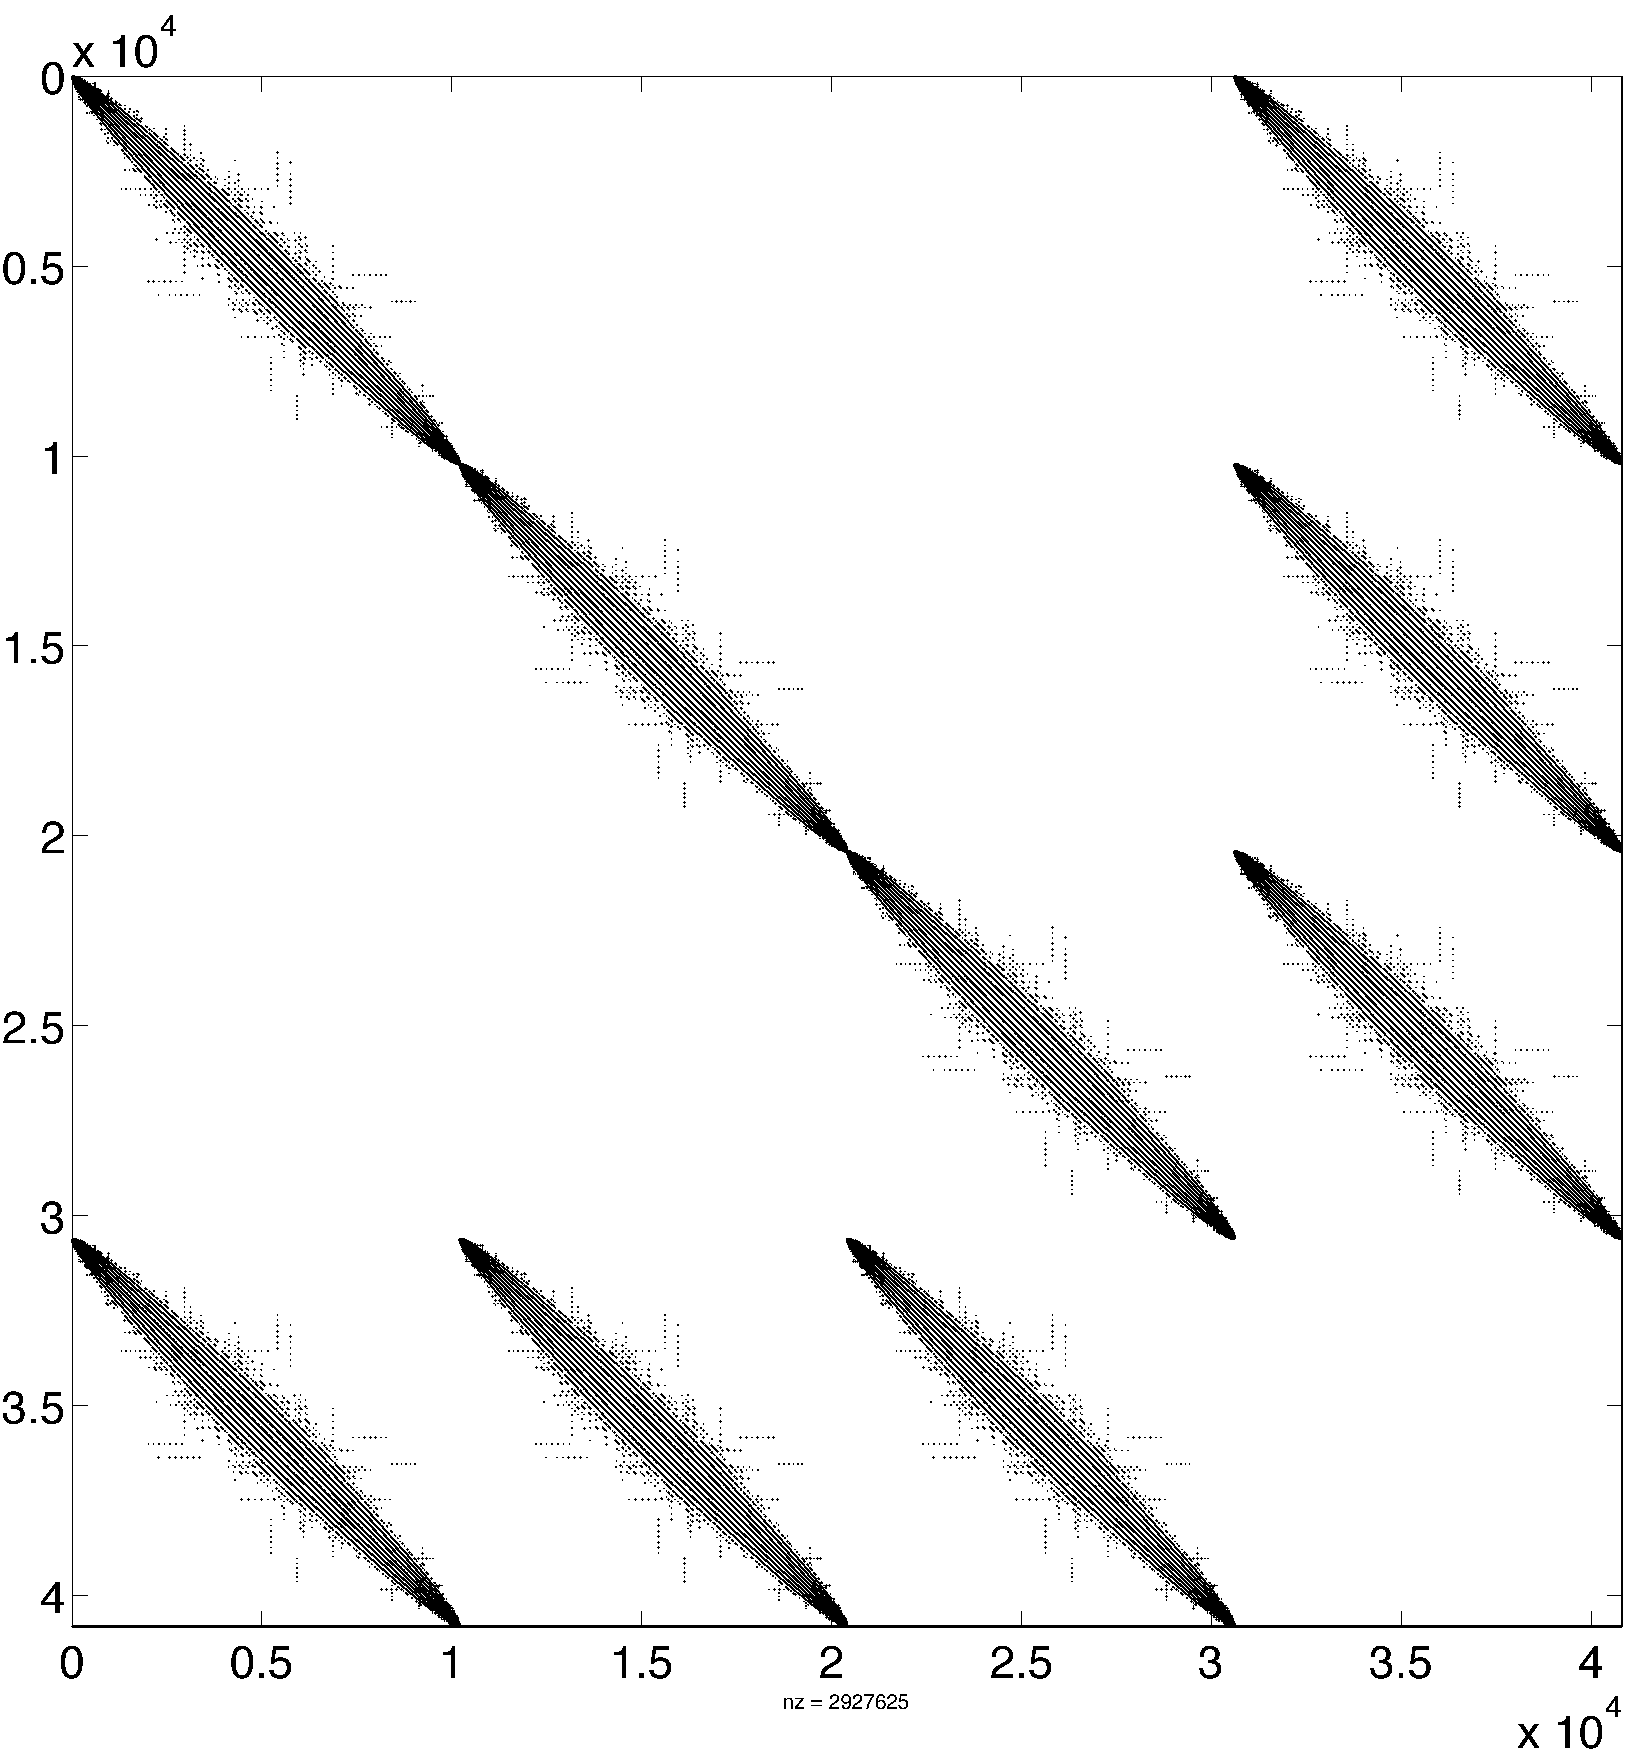
\includegraphics[width=1.0\textwidth]{figures/paper2/figures/N10201_KDTree_Stokes.pdf} 
		\caption{Grouped by Solution Component}
		\label{fig:original_stokes_dm}
	\end{subfigure}
	\begin{subfigure}[b]{0.4\textwidth}
		\centering
		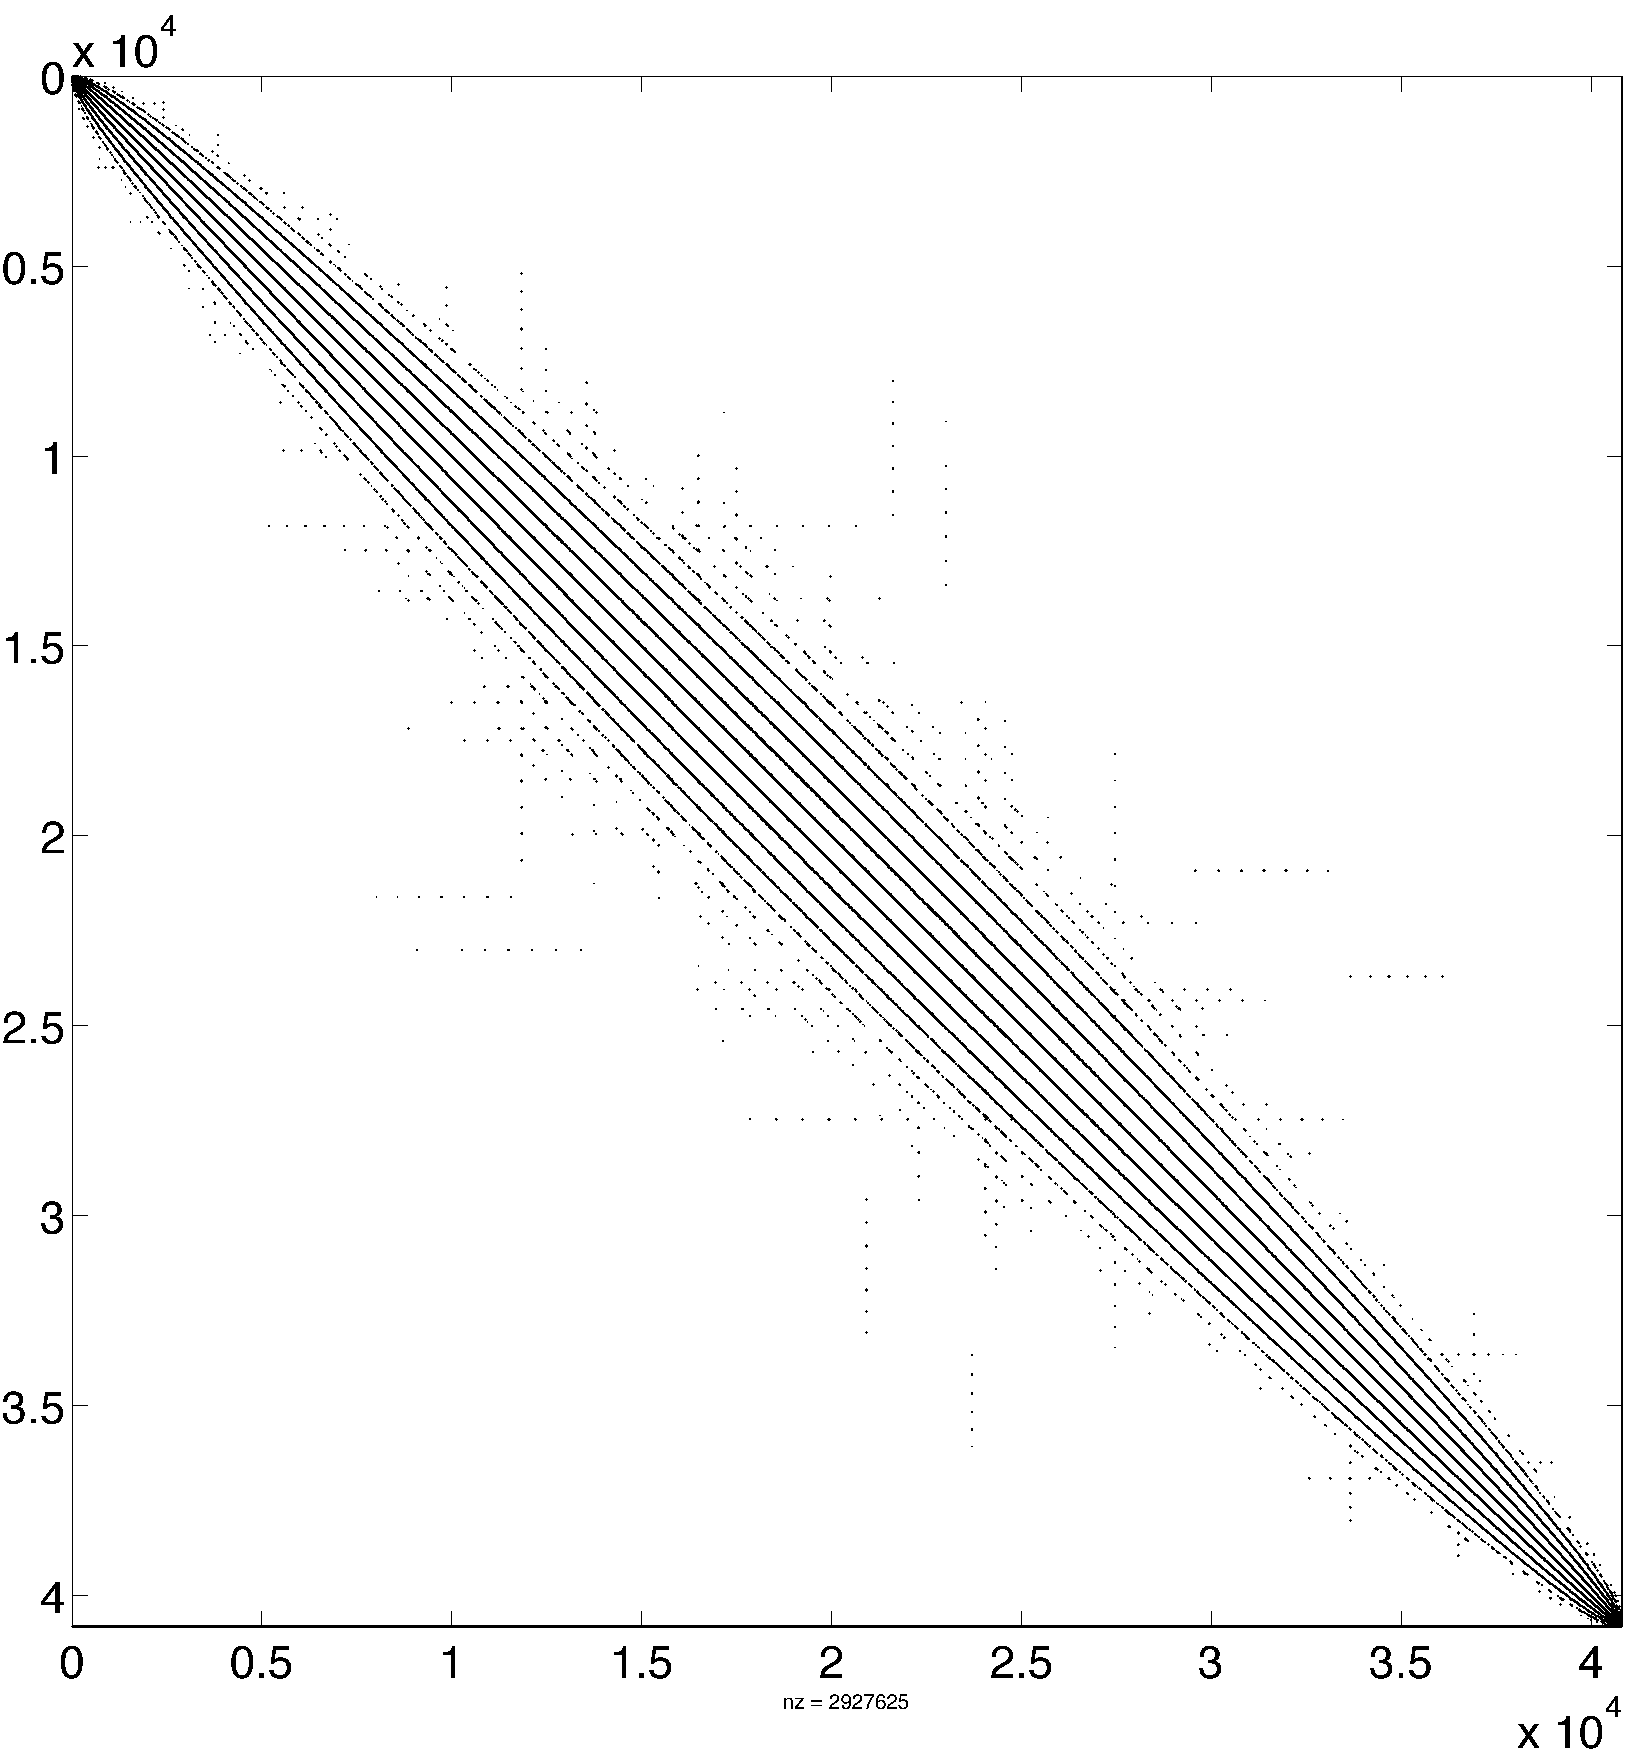
\includegraphics[width=1.0\textwidth]{figures/paper2/figures/N10201_KDTree_ReorderedStokes.pdf} 
		\caption{Interleaved Solution Components}
		\label{fig:interleaved_stokes_dm}
	\end{subfigure} \\
	\begin{subfigure}[b]{0.4\textwidth}
        		\centering
		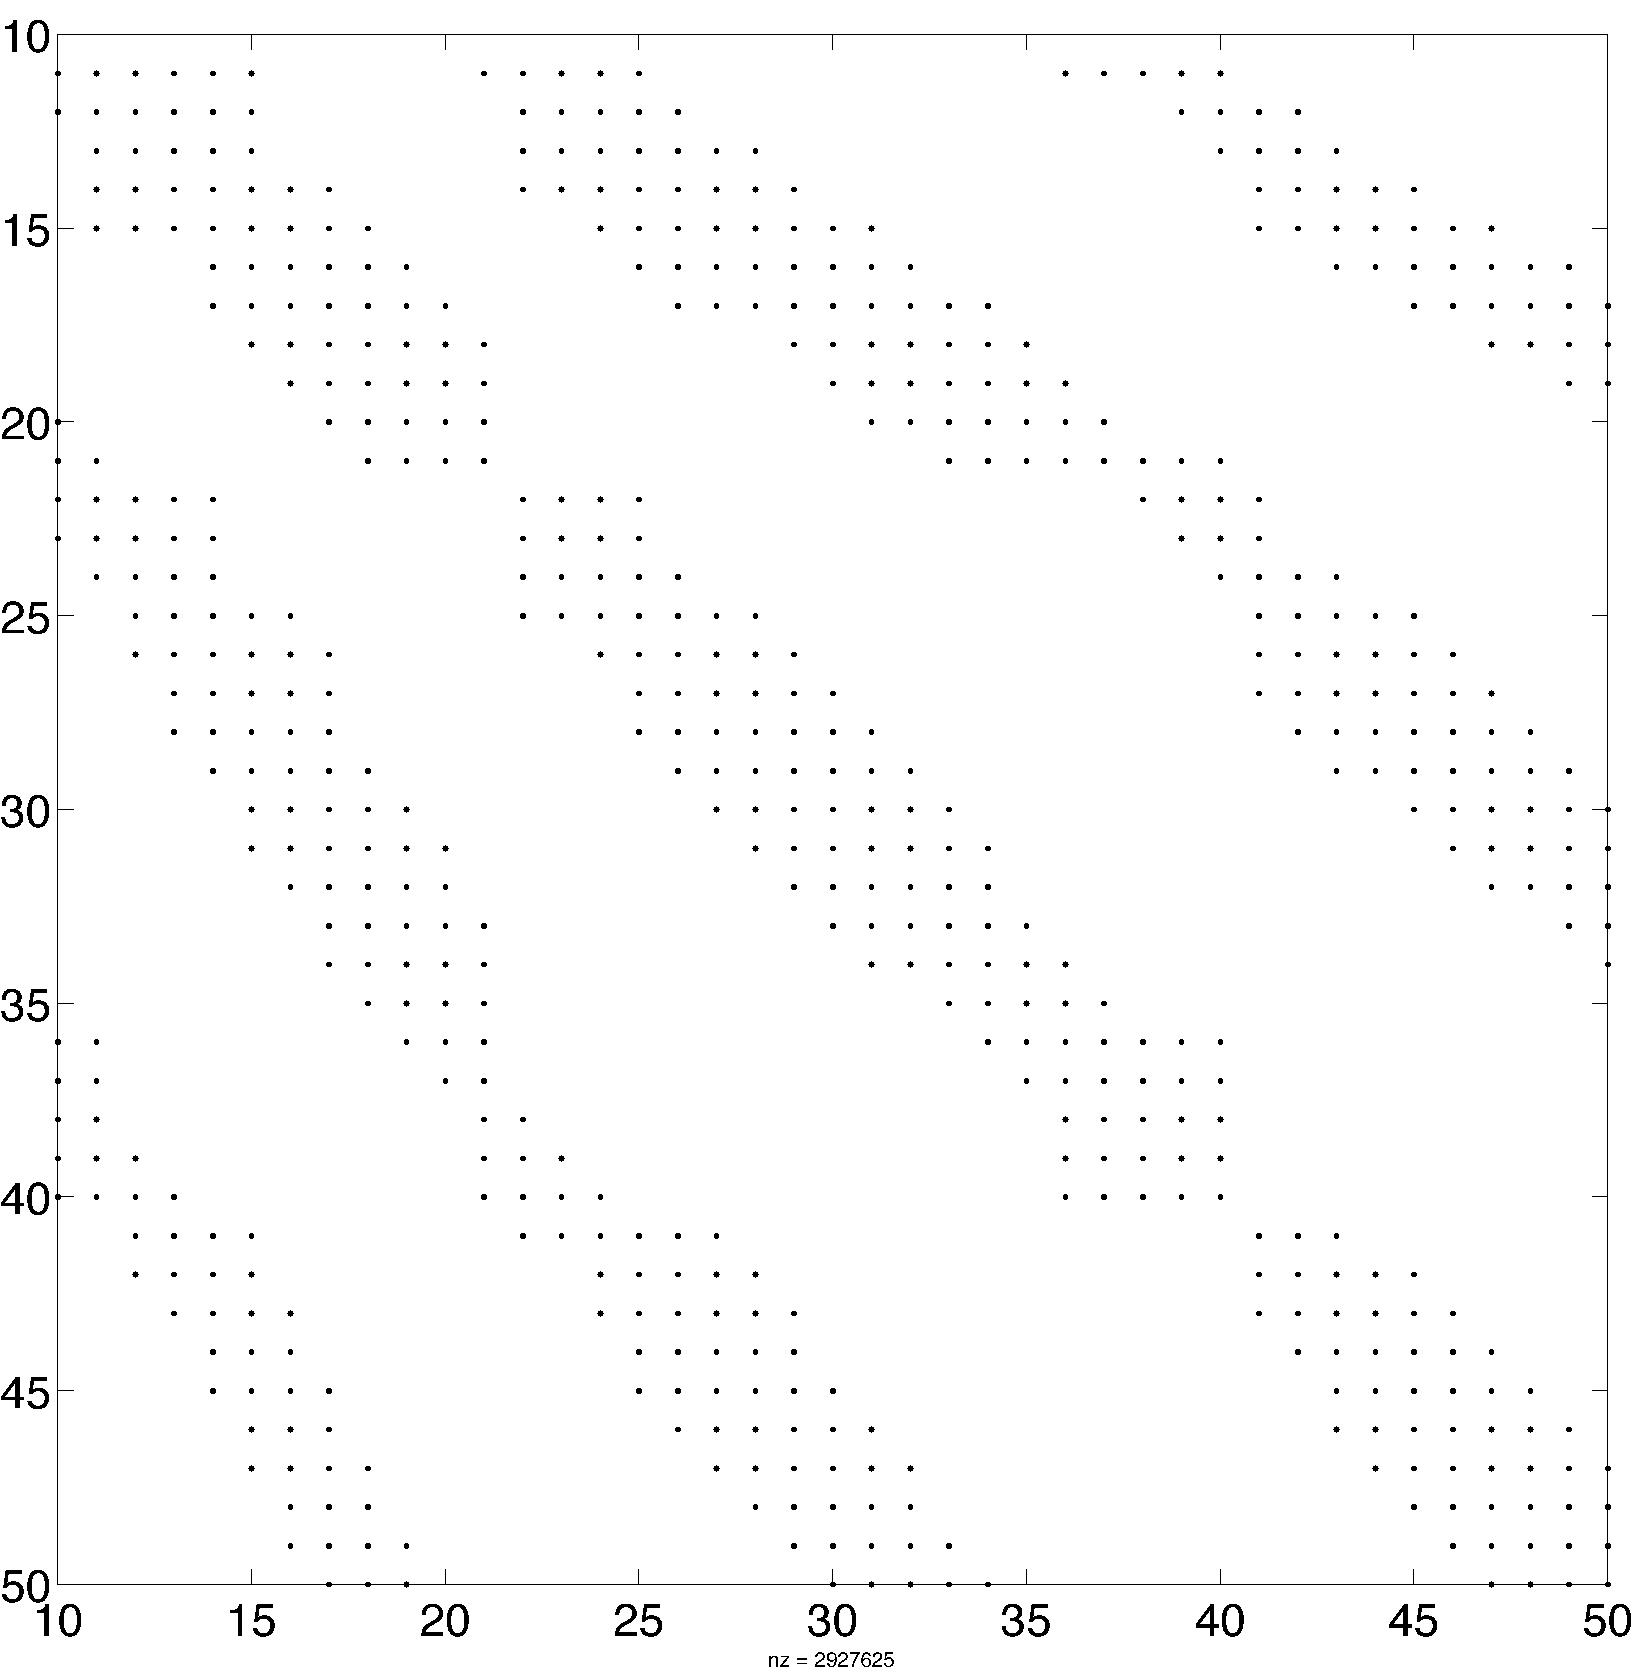
\includegraphics[width=1.0\textwidth]{figures/paper2/figures/N10201_KDTree_Stokes_10to50.pdf}
		\caption{Grouped Submatrix $(10:50) \times (10:50)$}
		\label{fig:original_stokes_zoom_dm}
	\end{subfigure}
	\begin{subfigure}[b]{0.4\textwidth}
		\centering
	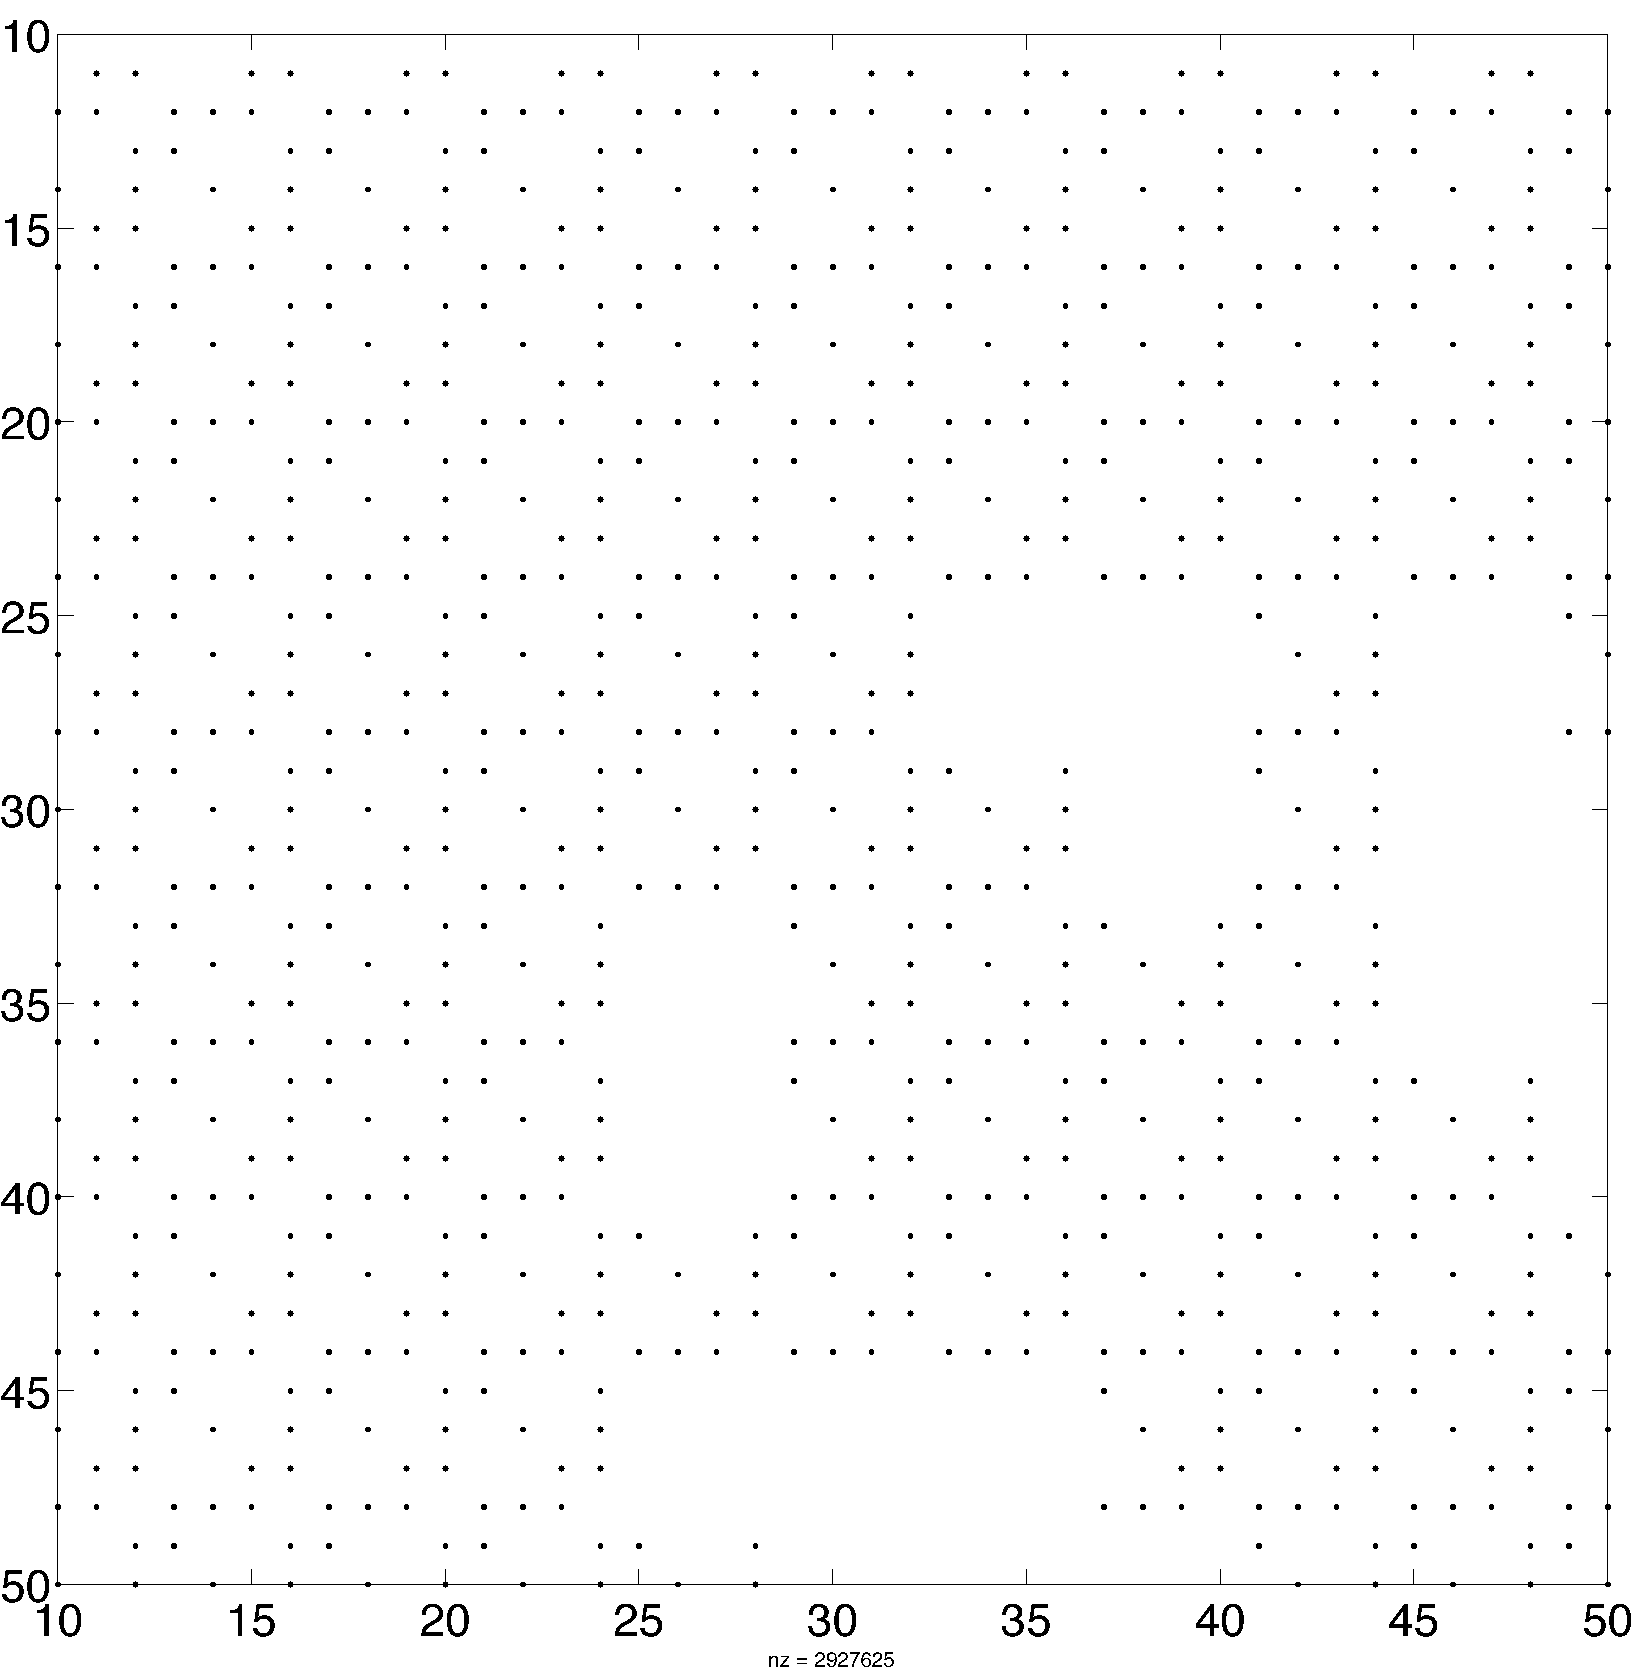
\includegraphics[width=1.0\textwidth]{figures/paper2/figures/N10201_KDTree_ReorderedStokes_10to50.pdf} 
		\caption{Interleaved Submatrix $(10:50) \times (10:50)$}
		\label{fig:interleaved_stokes_zoom_dm}
	\end{subfigure} \\
\caption{Sparsity pattern of linear system in Equation~\ref{eq:stokes_constant_viscosity}. Solution values are either ordered by component (e.g., $( u_1, \cdots, u_N, v_1, \cdots, v_N, w_1, \cdots, w_N, p_1, \cdots, p_N)^T$) or interleaved (e.g., $( u_1, v_1, w_1, p_1,\cdots, u_N, v_N, w_N, p_N)^T$). }
\label{fig:interleaved_solution}
\end{figure} 


\subsubsection{Node Order} 
\authnote{Should we discuss node ordering and its implications on convergence?}  
if so, I should state: 
\begin{itemize} 
\item Nodes are read from file
\item Their order is either: unmodified or modified
\item If modified, our goal is to improve memory access patterns by reducing the bandwidth of the DM. A bandwidth of $n$ is the best case scenario where the solution vector is accessed linearly. The worst case scenario is when bandwidth is $N$ and the solution is accessed randomly via stencils. 
\item Ordering nodes according to a space filling curve can reduce the ``randomness" of solution access by placing elements of stencils nearby (sometimes sequential) in memory. 
\item Many space filling curves exist. Raster (IJK), Snake, Morton, Hilbert, U, X, etc. We consider Raster here, with other orderings left for future work. 
\item Our restriction operator for domain decomposition might reduce the bandwidth for each processor compared to the global DM. How does the combination of restriction and reordering work? 
\item Reordering the DM has implications on its condition number and the convergence rate of the GMRES algorithm. We should provide bandwidth of matrix before and after reordering, as well as the condition number before and after. We should monitor convergence with and without reordering, and compare the number of GMRES iterations per minute/second. 
\end{itemize}  

\subsubsection{MPI Communication} 
The majority of communication within our implementation consists of two MPI routines: MPI\_Alltoallv and MPI\_Allreduce. 


\section{Governing Equations} 

We solve the PDE on the surface of the sphere as an example for one and multiple GPUs. Boundary conditions detract from the accuracy of RBF-FD and introduce other issues such as Runge phenomena \cite{RBFRungePaper}, so we first verify the solution without boundaries. 

%Viscous Stokes flow is described by the governing equations
%	\begin{align}
%\div{\vu} & = 0 \ \ \ \ \ \ \ \ \ \ \ \ \ \textsl{(Continuity)} \label{eq:stokes_continuity} \\
%\div{[\eta(\grad{\vu} + (\grad{\vu})^T)]} + Ra T \hat{r} & = \grad{p} \ \ \ \ \ \ \ \ \ \ \textsl{(Momentum)} \label{eq:stokes_momentum} \\
%\pd{T}{t} + (\vu \cdot \grad) T & = \Laplacian T \ \ \ \ \ \ \ \ \textsl{(Energy)}\label{eq:stokes_energy}
%\end{align}
%where the unknowns $\vu$ and $p$ represent the vector velocity- and scalar pressure-field respectively, $\eta$ is the viscosity tensor, $Ra$ is the non-dimensional Rayleigh number, and $T$ is the temperature profile. The focus of this paper is on the the implicit solve for Stokes flow, which amounts to the steady-state problem described by Equations~\ref{eq:stokes_continuity} and \ref{eq:stokes_momentum}. See \cite{Wright2010} for discussion of RBFs applied to the transient problem. 

\authnote{ Need to reference work that solves problem in two steps and justify our approach to solve in one step. Golub paper might be good for this. Or the Stoke preconditioners paper }

Assuming $\eta$ is a constant (i.e., $\grad\eta = 0$), our system simplifies to
\begin{align}
\begin{pmatrix}
-\eta \Laplacian & 0 & 0 & \pd{}{x_1} \\ 
0 & -\eta \Laplacian & 0 & \pd{}{x_2} \\ 
0 & 0 & -\eta \Laplacian & \pd{}{x_3} \\ 
\pd{}{x_1} & \pd{}{x_2} & \pd{}{x_3} & 0 \\
\end{pmatrix} \begin{pmatrix}
u_1 \\ u_2 \\ u_3 \\ p 
\end{pmatrix} = \frac{RaT}{\sqrt{x_1^2 + x_2^2 + x_3^2}}\begin{pmatrix} x_1 \\ x_2 \\ x_3 \\ 0\end{pmatrix}.
\label{eq:stokes_constant_viscosity}
\end{align}
where the $\Laplacian$ operator in spherical polar coordinates for $\mathbb{R}^3$ is: 
\begin{align} 
\Laplacian = \underbrace{\frac{1}{\hat{r}} \pd{}{\hat{r}} \left( \hat{r}^{2} \pd{}{\hat{r}}  \right)}_{\mathsf{radial}} + \underbrace{\frac{1}{\hat{r}^2} \Delta_{S}}_{\mathsf{angular}}. \label{eq:laplacian_in_spherical}
\end{align}
Here $\LaplaceBeltrami$ is the Laplace-Beltrami operator---i.e., the Laplacian constrained to the surface of the sphere with radius $\hat{r}$. This form nicely illustrates the components of the $\Laplacian$ corresonding to the radial and angular terms. 

On the surface of the unit sphere the radial term vanishes, so we are left with:
\begin{align}
\Laplacian    \equiv \LaplaceBeltrami . 
\end{align}
The following RBF operator from \cite{WrightFlyerYuen10}---Equation (20) can be applied to the RHS of Equation~\ref{eq:rbffd_weights} to generate Laplace-Beltrami RBF-FD weights: 
\begin{align} 
\LaplaceBeltrami = \frac{1}{4} \left[ \left(4-r^2\right) \pdd{}{r} + \frac{4-3r^2}{r} \pd{}{r} \right],
\end{align} 
where $r$ is the Euclidean distance between nodes of an RBF-FD stencil and is independent of our choice of coordinate system. 


Additionally following \cite{FlyerWright09, FlyerLehto11}, the off-diagonal blocks in Equation~\ref{eq:stokes_constant_viscosity} must be constrained to the sphere via the projection matrix: 
%\frac{1}{||\mathbf{x}||}
\begin{align}
P = I - \mathbf{x} \mathbf{x}^T =  \begin{pmatrix} 
(1-x_1^2) & -x_1 x_2 & -x_1 x_3 \\
-x_1 x_2 & (1-x_2^2) & -x_2 x_3 \\ 
-x_1 x_3 & -x_2 x_3 & (1-x_3^2) 
\end{pmatrix} = \begin{pmatrix} P_{x_1} \\ P_{x_2} \\ P_{x_3} \end{pmatrix}
\label{eq:project_gradient}
\end{align}
where $\mathbf{x}$ is the unit normal at the stencil center, and 
%
%Using the chain rule, and assumption that $r(\vx_k-\vx)=\vectornorm{\vx_k-\vx} = \sqrt{(x_{1,k}-x_1)^2 + (x_{2,k}-x_2)^2 + (x_{3,k}-x_3)^2}$, we obtain the unprojected gradient of $\phi$ as
%$$\nabla \phi(r(\vx_k - \vx)) = \pd{r}{\vx} \pd{\phi(r(\vx_k - \vx))}{r} = - (\vx_k - \vx)\frac{1}{r(\vx_k - \vx)} \pd{\phi(r(\vx_k - \vx))}{r}$$. 
%
%Applying the projection matrix gives 
%\begin{align}
%\mathbf{P} \nabla \phi(r(\vx_k - \vx)) & = - (\mathbf{P} \cdot \vx_k - \mathbf{P}\cdot\vx)\frac{1}{r(\vx_k - \vx)} \pd{\phi(r(\vx_k - \vx))}{r} =  - (\mathbf{P}\cdot\vx_k - 0)\frac{1}{r(\vx_k - \vx)} \pd{\phi(r(\vx_k - \vx))}{r} \\
%& = - (I-\vx\vx^T)(\vx_k
%)\frac{1}{r(\vx_k - \vx)} \pd{\phi(r(\vx_k - \vx))}{r} \\
%& = \begin{pmatrix} x \vx^T \vx_k - x_k \\ y \vx^T \vx_k -  y_k \\ z \vx^T \vx_k -z_k \end{pmatrix} \frac{1}{r(\vx_k - \vx)} \pd{\phi(r(\vx_k - \vx))}{r} 
% \end{align}
\cite{FlyerWright09, FlyerLehto11} show that with a little manipulation weights can be directly computed with these operators for Equation~\ref{eq:rbffd_weights}: 
%\begin{align} 
%P\pd{}{x_1} = ( x_1 \vx^T \vx_k - x_{1,k}) \frac{1}{d(\vx_k - \vx)} \pd{\phi(d(\vx_k - \vx))}{d} |_{\vx=\vx_j} \\
%P\pd{}{x_2} = ( x_2 \vx^T \vx_k - x_{2,k}) \frac{1}{d(\vx_k - \vx)} \pd{\phi(d(\vx_k - \vx))}{d} |_{\vx=\vx_j} \\
%P\pd{}{x_3} = ( x_3 \vx^T \vx_k - x_{3,k}) \frac{1}{d(\vx_k - \vx)} \pd{\phi(d(\vx_k - \vx))}{d} |_{\vx=\vx_j}
%\end{align}
\begin{align} 
P\pd{}{x_1} = ( x_1 \vx^T \vx_k - x_{1,k}) \frac{1}{r} \pd{}{r} |_{\vx=\vx_j} \\
P\pd{}{x_2} = ( x_2 \vx^T \vx_k - x_{2,k}) \frac{1}{r} \pd{}{r} |_{\vx=\vx_j} \\
P\pd{}{x_3} = ( x_3 \vx^T \vx_k - x_{3,k}) \frac{1}{r} \pd{}{r} |_{\vx=\vx_j}
\end{align}


\subsection{Constraints} 
Due to the lack of boundary conditions on the sphere, the family of solutions that satisfy the PDE in Equation~\ref{eq:stokes_constant_viscosity} includes four free constants (one for each $u_1$, $u_2$, $u_3$ and $p$). 
%In light of this, Equations~\ref{eq:stokes_linear_system} and \ref{eq:stokes_constant_viscosity} are singular with a four-vector null space corresponding to each for the four components of the solution $\begin{pmatrix} u_1, u_2, u_3, p \end{pmatrix}$. 

%The null space is found using the matlab sparse SVD command: \begin{mcode}{1}
%[Usvd, Ssvd, Vsvd, flagSVD] = svds(LHS,10,0);
%sing_value_indices = find(max(Ssvd) < 1e-6)
%\end{mcode} 

One way to close the null-space of the solution is to augment Equation~\ref{eq:stokes_constant_viscosity} with the following constraints: 
\begin{align}
\left(\begin{array}{cccc:cccc}  
-\eta \Laplacian & 0 & 0 & \pd{}{x_1} & 1_{N \times 1} & 0 & 0 & 0 \\ 
0 & -\eta \Laplacian & 0 & \pd{}{x_2} & 0 & 1_{N \times 1} & 0 & 0\\ 
0 & 0 & -\eta \Laplacian & \pd{}{x_3} & 0 & 0 & 1_{N \times 1} & 0\\ 
\pd{}{x_1} & \pd{}{x_2} & \pd{}{x_3} & 0 & 0 & 0 & 0 & 1_{N \times 1}\\
\hdashline
1_{1 \times N} & 0 & 0 & 0 & \multicolumn{4}{c}{\multirow{4}{*}{$0_{4 \times 4}$}} \\
0 & 1_{1 \times N} & 0 & 0 & \\
0 & 0 & 1_{1 \times N} & 0 & \\ 
0 & 0 & 0 & 1_{1 \times N} & \\
\end{array} \right) \left(\begin{array}{c} 
u_1 \\ u_2 \\ u_3 \\ p \\ \hdashline c_1 \\ c_2 \\ c_3 \\ c_4
\end{array} \right) = \frac{RaT}{\sqrt{x_1^2 + x_2^2 + x_3^2}}\begin{pmatrix} x_1 \\ x_2 \\ x_3 \\ 0 \\ \hdashline \int_\Omega u_1 \partial\Omega \\ \int_\Omega u_2 \partial\Omega \\ \int_\Omega u_3 \partial\Omega \\ \int_\Omega p \partial\Omega \end{pmatrix}.
\label{eq:stokes_system_with_constraints}
\end{align}
\authnote{Need the integral of my manufactured solution on the RHS. $\ell_1$ norm does not converge to 0, so it will screw solve with constraints}
where the subscript on $1_{N \times 1}$ indicates a $N \times 1$ vector of ones. These constraints add the unknowns $(c_1, c_2, c_3, c_4)$, which should solve to be zero. The four rows on the bottom require that the solution satisfy the integral over the domain for each solution component. In combination with the four added columns, the constraints indicate that the solution components must satisfy integrals using the same constant value. This is only possible if the constants are zero. Our added constraints are not chosen for physical significance, but for algebraic significance. When solving Equation~\ref{eq:stokes_system_with_constraints} with GMRES, the constraints improve conditioning of the system and increase the rate of convergence. 

We also investigate the use of GMRES without constraints. This increases the number of iterations required to converge, but allows increased parallelism (decreased data sharing). \authnote{Perhaps we can iterate without constraints until convergence slows then ``restart" the problem on a single GPU with constraints included? Limits scalability but would allow more parallelism for part of iterations while also reasonable convergence.}

\subsection{Manufactured Solution}

To verify our implementation, we manufacture a solution that satisfies the continuity equation. Using the identity
\begin{align} 
\div (\curl g(\vx)) = 0,
\end{align} 
for any function $g(\vx)$, we can easily manufacture a solution by choosing some vector function $g(\vx)$, projecting it onto the sphere via $P_x g(x)$ and applying the curl projection, $Q_x$: 
\begin{align} 
Q_x = \begin{bmatrix} 0 & -x_3 & x_2 \\ x_3 & 0 & -x_1 \\ -x_2 & x_1 & 0 \end{bmatrix}.
\end{align} 
Then, a manufactured solution that satisfies both momentum and continuity conditions on the surface of the sphere is given by: 
\begin{align} 
\vu = Q_x (g(\vx))
\end{align} 

Typically, on the surface of the sphere, the projection operator from Equation~\ref{eq:project_gradient} must be applied to an arbitrary $g(\vx)$. 
Here, we choose the components of $g(\vx)$ to be various spherical harmonics in Cartesian coordinates where $P_x Y_l^m = Y_l^m$. Consequently, application of $P_x$ can be ignored. 

We select $g(x)$ to be: 
\begin{align}
g(x) = 8 Y_{3}^{2} - 3Y_{10}^{5} + Y_{20}^{20} 
\end{align}
and the pressure function:
\begin{align}
P = Y_6^4 
\end{align} 

The manufactured solution is shown in Figure~\ref{fig:manufactured_solution}. A Mollweide projection \cite{Mollweide_ref} maps the sphere onto the plane. 

\begin{figure} 
\centering
\subfloat[Solution $Q_x( g(x) )$ with $g(x) = 8 Y_{3}^{2} - 3Y_{10}^{5} + Y_{20}^{20}$]{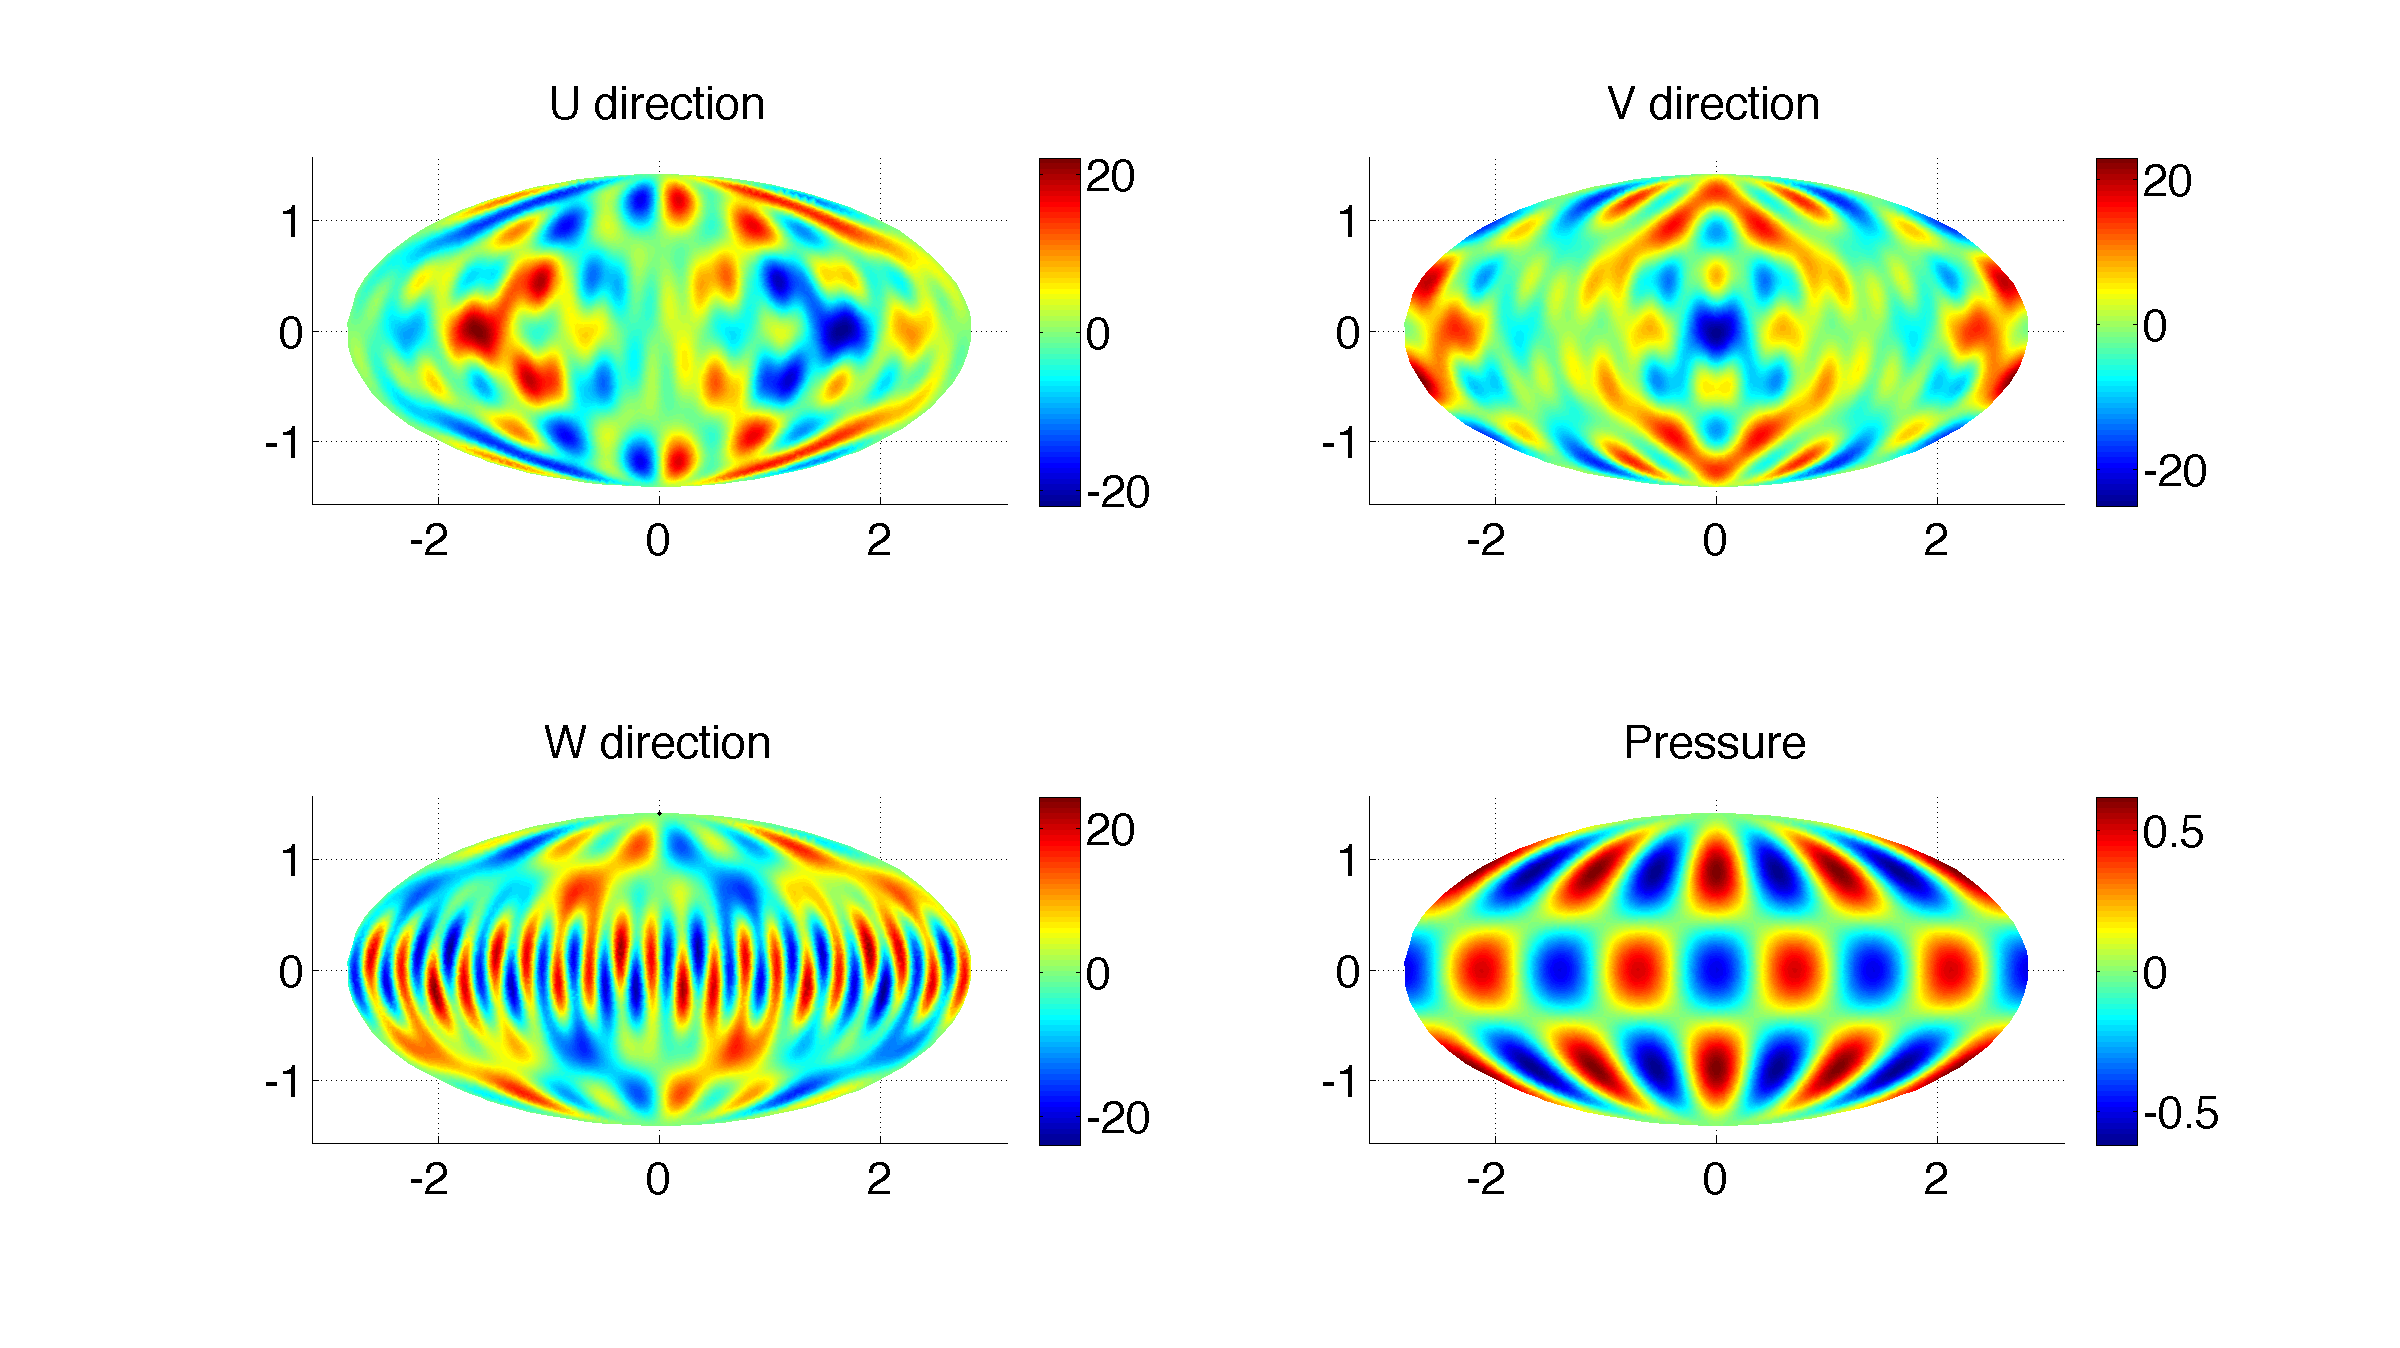
\includegraphics[width=1.0\textwidth]{figures/paper2/figures/U_exact.png}} \\
\subfloat[Right Hand Side (Constant Viscosity)]{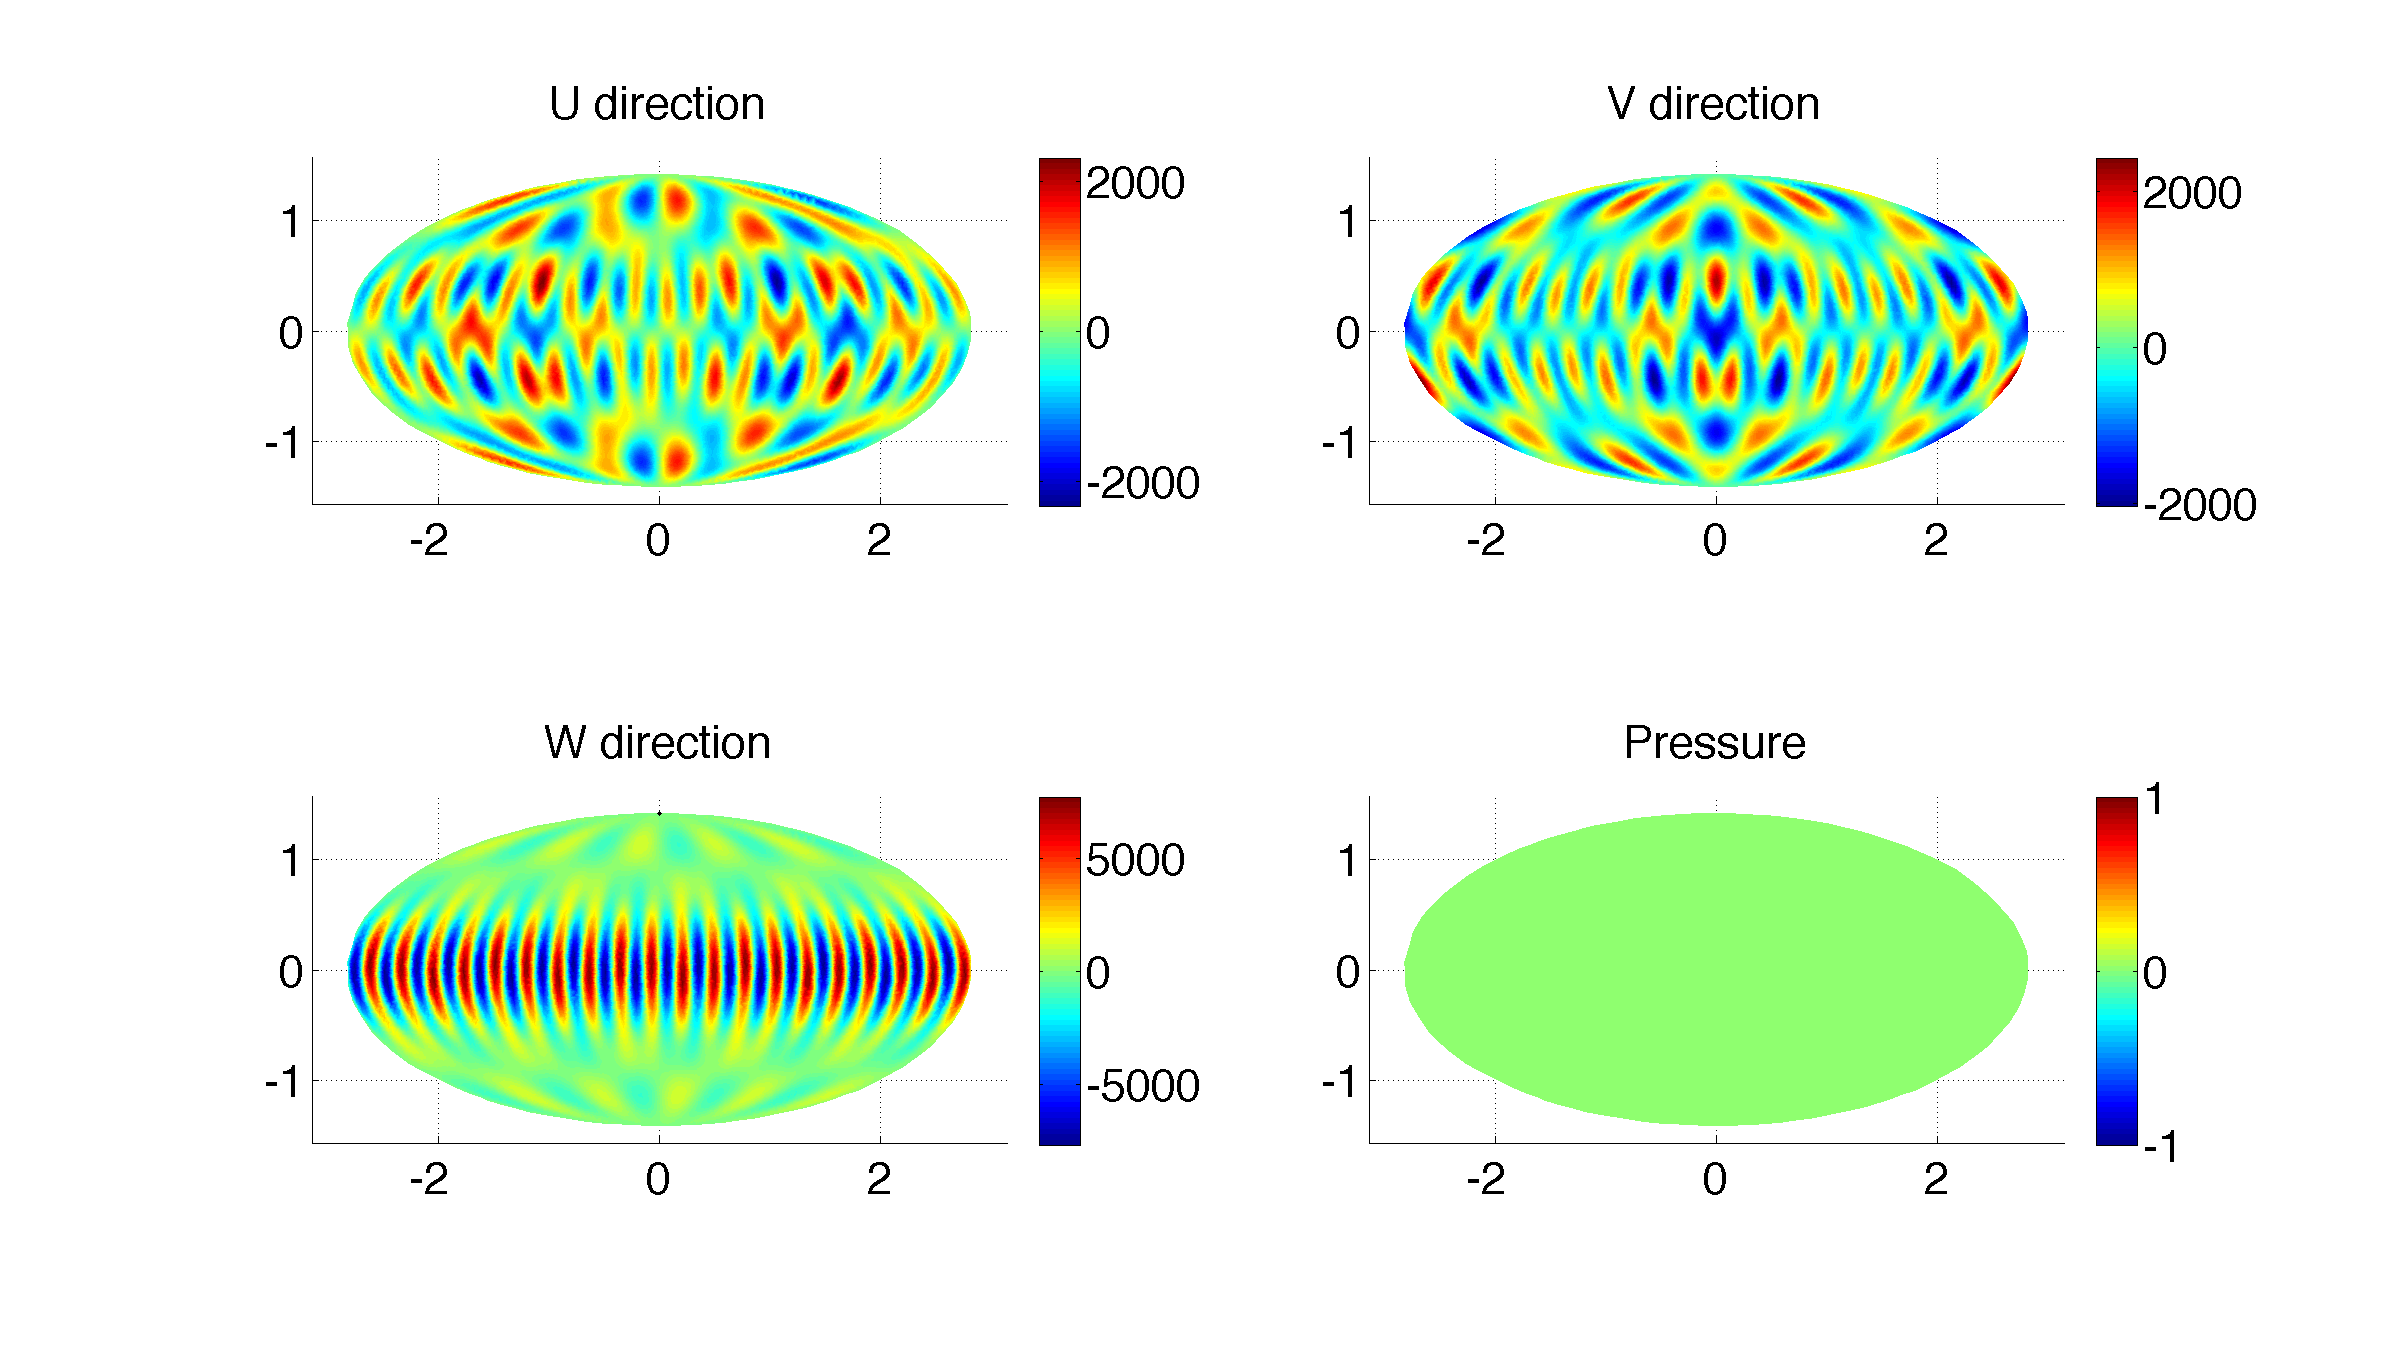
\includegraphics[width=1.0\textwidth]{figures/paper2/figures/RHS.png}}
\caption{A divergence free field is manufactured for the sphere. }
\label{fig:manufactured_solution}
\end{figure} 

\subsubsection{Convergence}

As the problem size $N$ increases, we expect the approximation to the solution to converge on the order of $\sqrt{n}$ where $n$ is the choice of stencil size. Figure~\ref{fig:convergence} demonstrates the convergence of our solution with respect to $\sqrt{N}$ for stencil sizes $n=31$,$101$ \authnote{update when figure is complete}. 




\section{Preconditioning} 

GMRES is slow to converge when used without a preconditioner. 

The differentation matrix produced by RBF-FD is asymmetric, non-positive definite, and non-diagonally dominant. Thus, many of the popular choices for preconditioning provided by CUSP and ViennaCL do not apply. 

Our tests show that an incomplete LU factorization with zero fill-in \cite{Saad2003} functions well. 

We also find that a large Krylov subspace must be saved. GMRES converges best when approximately 250 dimensions are saved between restarts. 

{\color{blue} Plot comparing residual of GMRES without precond and with ILU0 }

\authnote{ Need to comment on the conditioning of the system and how stencils can influence convergence }.
%\authnote{So my matlab code also demonstrates the behavior I was seeing in C++. The $n=31$ case converges VERY quickly with ILU0. However $n=40$ is slow. Another case that works well is $n=110$. I will have to go back and figure out how Im generating the stencils differently. I wonder if the $log(\kappa) = 14$ for $n=40$ is pushing conditioning too high to use? }

Need a table/plot comparing convergence of various preconditioners (ILU0, ILUT, AMG, etc.). We will justify our use of ILU0 even if it is the most basic and frequently least beneficial approach.

Demonstrate ILU0 is best for converging between 
\begin{itemize}
\item Jacobi
\item ILU0 on block $(1:3*N)$
\item ILU0 on full matrix
\item ILUT
\item AMG 
\end{itemize} 

\begin{algorithm}                     
\caption{Incomplete LU Factorization with Zero Fill-in (ILU0)}         
\label{alg:gmres}                        
\begin{algorithmic}[1]                  
    \For i = 0
    \State $a_{i,i} = a_{i,i} / a_{i,i}$
    \EndFor
\end{algorithmic}
\end{algorithm}

\section{GMRES Results}

We want to express benchmarks in terms of the number of GMRES iterations per second, and the number of iterations required to converge. Readers wont care what percentage of peak we are getting, just how fast we get to the solution. 

\begin{itemize} 
\item One GPU
\begin{itemize} 
	\item {\color{blue} Convergence for stokes steady}  
	\item {\color{blue} GMRES iteration plot (assuming 1e-8 and restart=60)} 
\end{itemize} 
\item Multi-GPU
	\begin{itemize} 
		\item Number of iterations without constraints
		\item Number of iterations with constraints
		\item GMRES iteration plot
		\item plot: number of GMRES iterations per second w.r.t. number of processors
	\end{itemize} 
\end{itemize} 


\section{Fragments}
Need to describe the solver. 

State that the conditions under which a problem is solved determines how quickly it will converge. For example, nodes too close together on delaunay meshes cause higher condition numbers and require more iterations. Proper choice of preconditioners can dramatically reduce the number of iterations required to converge. Although preconditioners incur an additional cost in preprocessing and at each iteration of the solver, 